\documentclass[12pt]{article}
\usepackage[spanish]{babel}
\usepackage{natbib}
\usepackage{url}
\usepackage[utf8x]{inputenc}
\usepackage[mediumspace,mediumqspace,Grey,squaren]{SIunits}
\usepackage{amsmath}
\usepackage{graphicx}
\graphicspath{{images/}}
\usepackage{parskip}
\usepackage{fancyhdr}
\usepackage{vmargin}
\usepackage{textcomp}
\setmarginsrb{3 cm}{2.5 cm}{3 cm}{2.5 cm}{1 cm}{1.5 cm}{1 cm}{1.5 cm}

\title{Constatación de instrumentos}								% Title
\author{Bosse-Bruno-Massitti}								% Author
\date{\today}											% Date

\makeatletter
\let\thetitle\@title
\let\theauthor\@author
\let\thedate\@date
\makeatother

\pagestyle{fancy}
\fancyhf{}
\rhead{\theauthor}
\lhead{\thetitle}
\cfoot{\thepage}

\begin{document}

%%%%%%%%%%%%%%%%%%%%%%%%%%%%%%%%%%%%%%%%%%%%%%%%%%%%%%%%%%%%%%%%%%%%%%%%%%%%%%%%%%%%%%%%%

\begin{titlepage}
	\centering
    \vspace*{0.5 cm}
    
\includegraphics[scale = 0.45]{utn_logo.jpg}\\[1.0 cm]	% University Logo
    \textsc{\LARGE Universidad Tecnológica Nacional}\\[2.0 cm]	% University Name
	\textsc{\Large Curso 4R2}\\[0.5 cm]				% Course Code
	\textsc{\large Medidas Electrónicas I}\\[0 cm]				% Course Name
	\textrm{\large (Ing. Salamero e Ing. Centeno)}\\[0.5 cm]
    \rule{\linewidth}{0.2 mm} \\[0.4 cm]
	{ \huge \bfseries \thetitle}\\
	\rule{\linewidth}{0.2 mm} \\[1 cm]
	
	\begin{minipage}{0.4\textwidth}
		\begin{flushleft} \large
			\emph{Autores:}\\
			Esteban Bosse\\Luis Bruno\\Martín Massitti
			\end{flushleft}
			\end{minipage}~
			\begin{minipage}{0.4\textwidth}
			\begin{flushright} \large
			\emph{Legajo N:} \\
			 62.930\\57.760\\62.623									% Your Student Number
		\end{flushright}
	\end{minipage}\\[2 cm]
	
	{\large \thedate}\\[2 cm]
 
	\vfill
	
\end{titlepage}

%%%%%%%%%%%%%%%%%%%%%%%%%%%%%%%%%%%%%%%%%%%%%%%%%%%%%%%%%%%%%%%%%%%%%%%%%%%%%%%%%%%%%%%%%

\tableofcontents
\pagebreak

%%%%%%%%%%%%%%%%%%%%%%%%%%%%%%%%%%%%%%%%%%%%%%%%%%%%%%%%%%%%%%%%%%%%%%%%%%%%%%%%%%%%%%%%%

\section{Introducción}
En el tercer trabajo de laboratorio se planteo el diseño de un amplificador que cuenta con un transistor en configuración de colector común, el transistor empleado es el BC548C (Beta=398). Dicho practico tiene la función de analizar y comprender el trabajo del transistor en esta configuración.
\begin{figure}[ht]
\centering 
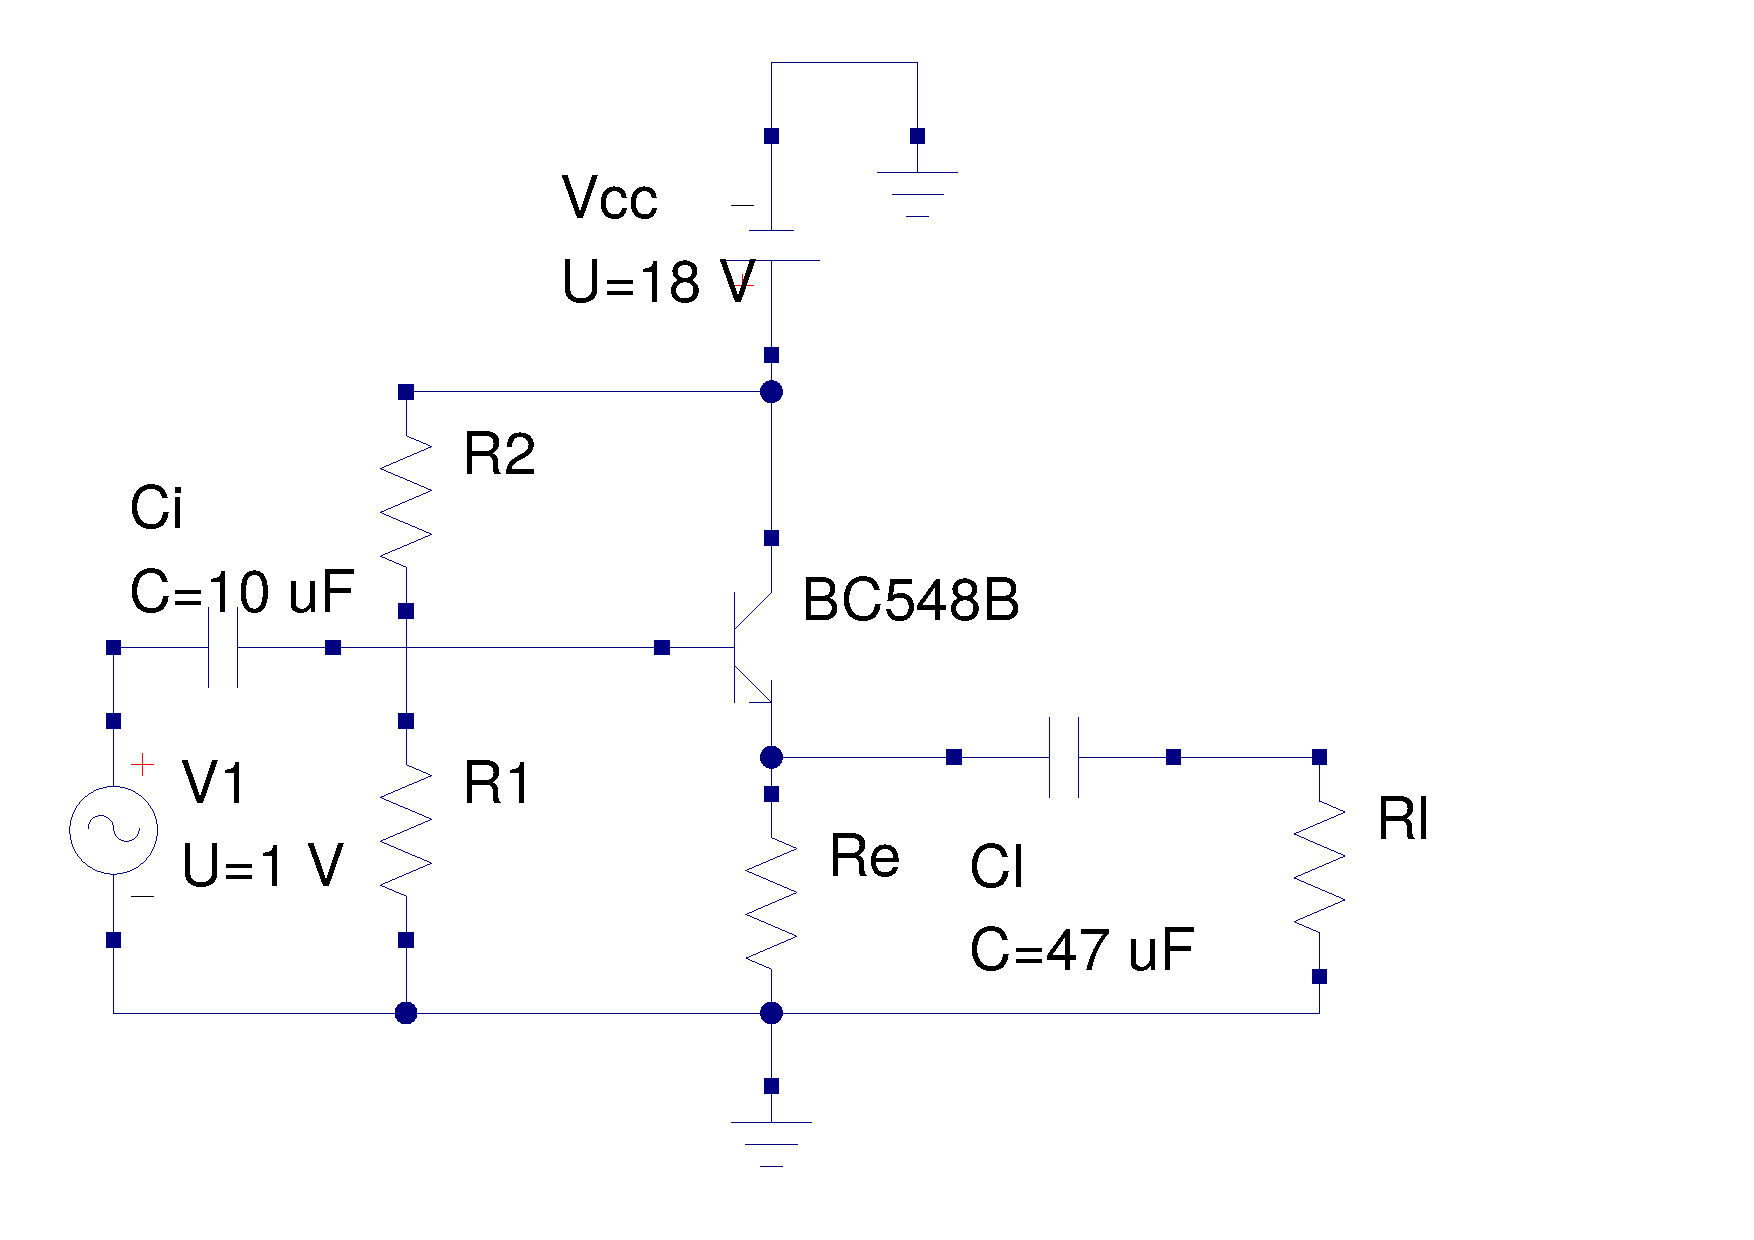
\includegraphics[scale = 0.5]{cc.pdf}\\[0.25 cm]	% Imagen Termistor
\caption{Colector Comun}
\label{Figura 1}
\end{figure}

\newpage
\section{Diseño para MES}
Como instancia inicial, utilizando la información proporcionada en clase, se realizó el calculo de $I_{CQMES}$ y $V_{CEQMES}$. 
\begin{equation}
\label{ICQMES}
I_{CQMES}=\dfrac{V_{CC}}{R_E+R_E//R_L}
\end{equation}
\begin{equation}
\label{VCEQMES}
V_{CEQMES}=V_{CC}-I_{CQMES}.R_E
\end{equation}
\underline{Datos:}

$R_E=1,5 K\Omega$
 
$R_L=1k\Omega$

$V_{CC}=18V$

$\beta = 398$ 

$C_I=10\micro F$

$C_L=47\micro F$
\subsection{Valores Exactos}
Citando la ecuaciones (\ref{ICQMES}) y (\ref{VCEQMES}) y reemplazando sus valores con los datos propuestos en clase, obtenemos:

\begin{equation}
\label{I_{CQMES}}
I_{CQMES}=\dfrac{18V}{1,5K\Omega+\dfrac{1,5k\Omega*1k\Omega}{1,5k\Omega+1k\Omega}}
\end{equation}
\vspace{0.2cm}
\begin{equation}
I_{CQMES}=8,571mA
\end{equation}

\begin{equation}
\label{V_{CEQMES}}
V_{CEQMES}=18V-\dfrac{18V}{1,5K\Omega+\dfrac{1,5k\Omega*1k\Omega}{1,5k\Omega+1k\Omega}}*1,5K\Omega
\end{equation}
\vspace{0.2cm}
\begin{equation}
V_{CEQMES}=5,145V 
\end{equation}

\newpage
\textbf{Thevenin}

El teorema establece que si una parte de un circuito eléctrico lineal está comprendida entre dos terminales A y B, esta parte en cuestión puede sustituirse por un circuito equivalente.
Utilizamos el teorema para obtener el valor de $R_B$ y $V_{BB}$.
\begin{equation}
 R_B=\dfrac{\beta R_E}{10}
\end{equation}
\begin{equation}
 V_{BB}=I_{CQMES}(R_E+\dfrac{R_B}{\beta})+0.7V
\end{equation}
Reemplazando los datos en las ecuaciones anteriores:
\begin{center}
$R_B=\dfrac{398*1,5K\Omega}{10}$

$R_B=50,7k\Omega$

\vspace{0.8 cm}
$V_{BB}=8,571mA(1,5k\Omega+\dfrac{50,7k\Omega}{398})+0.7$

$V_{BB}=14,842V$
\end{center}
\vspace{1 cm}
A partir de estas 2 ecuaciones podemos calcular $R_1$ y $R_2$,  estas resistencias nos permiten “independizar” al $I_{CQ}$ y $V_{CEQ}$ del beta del transistor (empleando un divisor de voltaje), ya que este es muy sensible a la temperatura y posee un valor particular para cada transistor. Logrando así una estabilidad en el circuito que permite hallar la recta de carga de una forma más exacta.
\begin{equation}
\label{R1}
 R_1=\frac{R_B}{1-\dfrac{V_{BB}}{V_{CC}}}
\end{equation}
\begin{equation}
\label{R2}
 R_2=\frac{R_B}{\dfrac{V_{BB}}{V_{CC}}}
\end{equation}
\vspace{0.5cm}
Reemplazando por los valores obtenidos:
\begin{center}
 
$R_1=\dfrac{50,7k\Omega}{1-\dfrac{14,842V}{18V}}$

$R_1=288,9k\Omega$

\vspace{0.8 cm}
$R_2=\dfrac{50,7k\Omega}{\dfrac{14,842V}{18V}}$

$R_2=61,48k\Omega$
\end{center}


\subsection{Valores Simulados y Normalizados}
Luego de los cálculos realizados, se procedió a la simulación para obtener valores aproximados de los datos, poder encontrar valores comerciales normalizados, llevar a cabo el circuito y realizar las mediciones pertinentes.
\begin{center}
 $R_E=1,5k\Omega$

 $R_1=330K\Omega$
 
 $R_2=68K\Omega$

 \end{center}

 
 



\subsection{Valores Reales}
Son los valores que obtuvimos al realizar las mediciones pertinentes en el circuito.
\begin{center}
  $I_{CQMES}=8,69mA$
  
  $V_{CEQMES}=5,169V$
  
  $V_{BB}=14,842V$
  

\end{center}

\section{Análisis y trazado de las rectas de carga para MES}
Si graficamos las rectas de corriente alterna y corriente continua, podemos observar que se intersectan en un punto, al que llamaremos punto Q. Este punto nos indica el punto medio de trabajo del transistor en la configuración propuesta. Podemos ver que las coordenadas del punto Q estan dadas por la Corriente en el colector y la tensión colector emisor, al igual que las rectas CC y CA.

\subsection{Recta de carga CC}
Para encontrar los extremos de la recta de carga:
\begin{equation}
  v_{CE}=V_{CC}-i_{C}R_E
\end{equation}
Para hallar $I_{C}$ hacemos $V_{CE}=0$
\begin{center}
  $i_{C max}=\frac{V{CC}}{R_E}$
  
  $i_{C max}=12,278mA$
\end{center}
Para encontrar $V_{CE}$ hacemos $I_C=0$
\begin{center}
  $v_{CE max}=V_{CC}$
  
  $v_{CE max}=18V$
\end{center}

 

\subsection{Recta de carga CA}

Para encontrar los extremos de la recta de carga:
\begin{equation}
  v_{CE}=V_{CC^{'}}-i_{C}(R_E//R_L)
\end{equation}

Para encontrar $v_{CE}$ hacemos $i_C=0$
\begin{center}
  $v_{CE max}=V_{CC^{'}}$
\end{center}

\begin{equation}
  V_{CC^{'}}=V_{CEQMES}+I_{CQMES}*R_E//R_L
\end{equation}
\begin{center}
 $V_{CC^{'}}=5.169V+8,69mA(\dfrac{1466\Omega+998\Omega}{1466\Omega*998\Omega})$
\vspace{0.2cm} 

$V_{CC^{'}}=10,328V$

\end{center}
  
Para hallar $i_{C}$ hacemos $v_{CE}=0$
\begin{center}
  $i_{C max}=\frac{V{CC^{'}}}{R_E//R_L}$
  
  $i_{C max}=\dfrac{10,328V}{\dfrac{1466\Omega*998\Omega}{1466\Omega+998\Omega}}$
\vspace{0.2cm} 

 $i_{C max}=17.39mA$
\end{center}

  
 \begin{figure}[ht]
\centering 
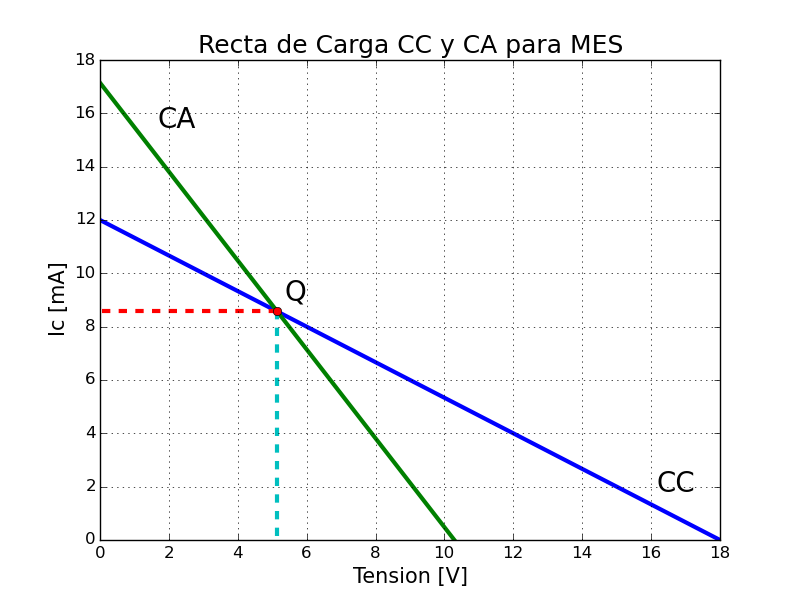
\includegraphics[scale = 0.6]{RectaCCCA.png}\\[0.25 cm]	% Imagen Termistor
\caption{Recta de Carga}
\label{Figura 5}
\end{figure}

\begin{center}

\subsection{Punto Q}
    
  $I_{CQMES}=8,69mA$

  $V_{CEQMES}=5,169V$
\end{center}


\section{Mediciones en pequeña señal}
Las mediciones de pequeña señal o tambien llamadas parámetros hibridos.
Son los parametros internos del transistor en alterna. Son cuatro parametros:

\begin{itemize}
\item Impedancia $Z$
\item Ganacia de tensión $\Delta V$
\item Ganacia de corriente $\Delta I$
\end{itemize}
En primer lugar realizamos el calculo de los parametros hibridos.
Colocamos una resistencia sensora $R_S$ de un valor de $33 k\Omega$. La función de esta resistencia es, medir la caida de tension que producia en el circuito y asi poder calcular la corriente que circulaba a traves de ella por la ley de Ohm.

\subsection{Impedancia de Entrada $Z_i$}
\begin{equation}
 Z_i=\dfrac{V_i}{\dfrac{V_G-V_i}{R_S}}
\end{equation}
Siendo $V_G=336mV$ y $V_i=190mV$:
\begin{center}
 $Z_i=\dfrac{324mV}{\dfrac{326mV-190mV}{32,61k\Omega}}$
 
 $Z_i=75,048K\Omega$
\end{center}

\subsection{Impedancia de Salida $Z_o$}
Para calcular la impedancia de salida aplicamos la señal en la salida del circuito, colocando la resistencia sensora de $R_S=10 \Omega$ , utilizamos una tension de $V_L=0,2V$ pico a pico, ya que con $1V$ habia demasiada distorsion.  .
\begin{equation}
 Z_o=\dfrac{V_o}{\dfrac{V_G-V_o}{R_S}}
\end{equation}
\begin{center}
 $Z_o=\dfrac{22mV}{\dfrac{60mV-22mV}{9,99\Omega}}$
 
 $Z_o=5,76\Omega$
\end{center}

\subsection{Ganancia de Tension $\Delta V$}
\begin{equation}
 \Delta V=\frac{V_L}{V_I}
\end{equation}
\vspace{0.2cm}
Aplicamos $0.2V$ pico a pico en $V_L$
\begin{center}
 $\Delta V=\dfrac{318mV}{336mV}$
 
 $\Delta V=0,9464$
\end{center}

\subsection{Ganancia de Corriente $\Delta I$}
\begin{equation}
  \Delta I=\frac{I_L}{I_I}=\dfrac{\dfrac{V_L}{R_L}}{\dfrac{V_G-V_I}{R_S}}
\end{equation}
\vspace{0.2cm}
\begin{center}
$\Delta I=\dfrac{\dfrac{318mV}{998\Omega}}{\dfrac{336mV-190mV}{9,99\Omega}}$

$\Delta I=71,16$
\end{center}


\section{Conclusiones}
Al realizar la experiencia en el laboratorio pudimos observar que los calculos no son muy exactos,al igual que en los otros practicos esto se debe a los multimetros y osciloscopios utilizados. Por otro lado observamos grandes variaciones en los valores de la resistencias,debido a la limitacion de utilizar valores comerciales normalizados.
Pudimos observar que al aplicar 1V pico a pico,obtuvimos una distorsion muy grande. Por lo cual tuvimos que utilizar una tension 0.2V pico a pico.
Cabe destacar que las mediciones de tension fueron efectuadas con el multimetro para obtener una mejor precision. Es destacable tambien la precision obtenida en la tension eficaz con los distintos instrumentos de medicion, debido el calculo de la tension rms.
Con los datos recopilados durante la experiencia podemos concluir que esta configuracion no posee ganacia de tensión(perdida), una buena ganacia de corriente, una alta impedancia de entrada y una baja impedancia de salida.
Siendo las impedancias opuestas a la configuracion de base comun.
\bibliographystyle{plain}
\bibliography{biblist}
Apuntes varios de clase.

\end{document}
